\begin{figure}[ht!]
\centering
	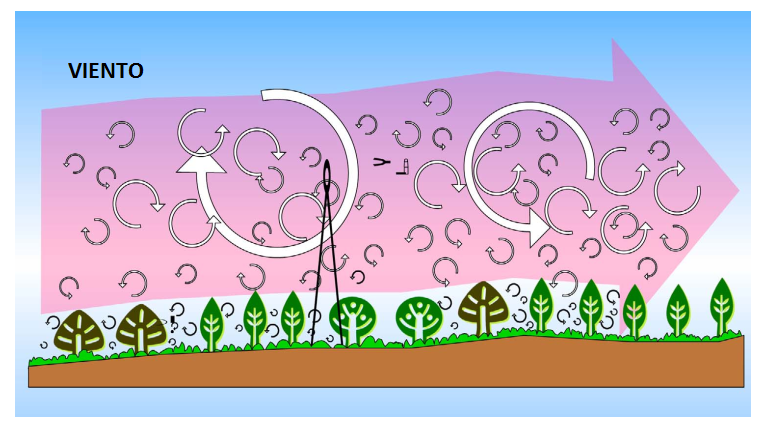
\includegraphics[scale=0.77]{Images/wang01.png}
	\caption{Vista esquemática del flujo de aire que puede ser visto como un flujo horizontal de numerosos remolinos giratorios, es decir, vórtices turbulentos de varios tamaños (con componentes horizontales y verticales).}
	{\raggedright FUENTE: \citet{wang2012review}.	 \par}

	\label{fig:wang01}
\end{figure}